\clearpage
\section{Project Roles}

Scrum defines three project roles — the product owner, the scrum master and the development
team. As this bachelor thesis is an academical project, the scrum roles could
not be mapped one to one. This Section introduces the involved persons and their roles
in the project.

\subsection{HSR Supervisor}

\begin{minipage}[t]{0.25\textwidth}
	\vspace{0pt}
	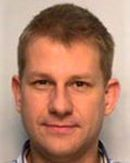
\includegraphics[width=0.8\textwidth]{olz.jpg}
\end{minipage}
\begin{minipage}[t]{0.8\textwidth}
	\vspace{10pt}
	Prof. Dr. Olaf Zimmermann is the \gls{HSR} supervisor of this thesis and incorporates both, the role of the product owner and scrum master. \textit{Product} in this context refers to the thesis itself as well as the functional product. He ensures that all requirements by HSR for a bachelor thesis are met and decides in last instance about the scope of the thesis. 
	As supervisor and coach of the development team, Mr. Zimmermann also performs part of the scrum master role as he coaches the development team.
\end{minipage}


\subsection{Industry Partner}

Our industry partner Zühlke Engineering, represented by W. Giersche, ensured the functional relevancy of this thesis. Mr. Giersche contributed valuable experience from many software engineering projects. He represented part of the product owner role as he played an important role in the functional prioritization to maximize the business value. Being an experienced software architect, he also contributed to the coupling criteria catalog by conducting workshops.


\subsection{Project Team}

Michael Gysel and Lukas Kölbener formed the development team. They worked as an interdisciplinary team in which both were responsible for each part of the project. Both being Certified ScrumMasters\textregistered\cite{scrummaster}, they incorporated part of the scrum master role as they helped maintaining the product backlog and organized everything for correct sprint operation.

\begin{minipage}[t]{0.25\textwidth}
	\vspace{0pt}
	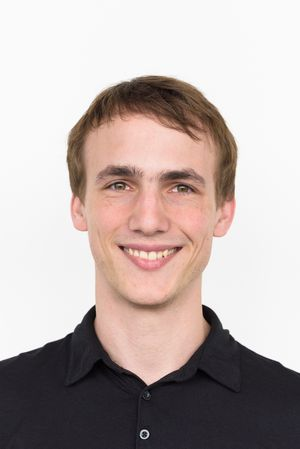
\includegraphics[width=0.8\textwidth]{lukas.jpg}
\end{minipage}
\begin{minipage}[t]{0.8\textwidth}
	\vspace{20pt}
	Lukas Kölbener is an information technology student at \gls{HSR} in his 9\textsuperscript{th} semester. He works part time as Java developer for Super Computing Systems AG in Zurich, building ticket vending machines for the public transport industry.
	\newline
\end{minipage}

\begin{minipage}[t]{0.25\textwidth}
	\vspace{0pt}
	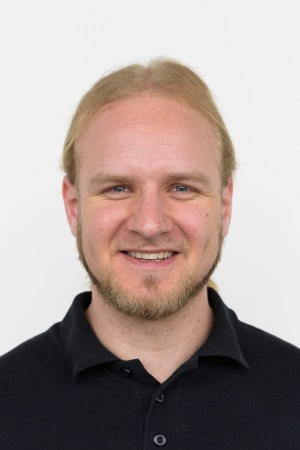
\includegraphics[width=0.8\textwidth]{michi.jpg}
\end{minipage}
\begin{minipage}[t]{0.8\textwidth}
	\vspace{20pt}
	Michael Gysel is an information technology student at \gls{HSR} in his 9\textsuperscript{th} semester. He works part time as Java Developer for FIS, a global provider for banking and payments technologies.
	\newline
\end{minipage}
